% Copyright 2004 by Till Tantau <tantau@users.sourceforge.net>.
%
% In principle, this file can be redistributed and/or modified under
% the terms of the GNU Public License, version 2.
%
% However, this file is supposed to be a template to be modified
% for your own needs. For this reason, if you use this file as a
% template and not specifically distribute it as part of a another
% package/program, I grant the extra permission to freely copy and
% modify this file as you see fit and even to delete this copyright
% notice. 

\documentclass[aspectratio=169, 12pt, fleqn]{beamer}

\usepackage{graphicx} 
\usepackage{animate}
\usepackage{listliketab}
%\usepackage{booktabs}% http://ctan.org/pkg/booktabs

\usepackage{../include/cs-seminar}
\usepackage{../include/lstcoq}
\usepackage{../include/lstisabelle}

%\usepackage{render_to_a4}

%\usepackage{tabularx}
\usepackage[normalem]{ulem}
\usepackage{mwe,tikz}

\lstset{ 
  frame=none,
  captionpos=t,
  basicstyle=\ttfamily\footnotesize,
}
\usepackage{caption}
\DeclareCaptionFont{ninept}{\fontsize{8pt}{11pt}\selectfont #1}
\captionsetup{singlelinecheck=false, font=ninept}
\renewcommand*\lstlistingname{Example}  % not Example, not Listing. See

% space saving tips: https://gist.github.com/yig/81b4c993ea13252edc81
\setlength\lineskip{0pt}
\setlength{\abovedisplayskip}{0pt}
\setlength{\belowdisplayskip}{0pt}
%\setlength\abovedisplayshortskip{0pt}
%\setlength\belowdisplayshortskip{0pt}
%\setlist{nosep}

% strikeout text : \hcancel[red]{text...}
\newcommand\hcancel[2][black]{\setbox0=\hbox{$#2$}%
\rlap{\raisebox{.45\ht0}{\textcolor{#1}{\rule{\wd0}{2pt}}}}#2}

% table space https://en.wikibooks.org/wiki/LaTeX/Tables
\renewcommand{\arraystretch}{0}
% There are many different themes available for Beamer. A comprehensive
% list with examples is given here:
% http://deic.uab.es/~iblanes/beamer_gallery/index_by_theme.html
% You can uncomment the themes below if you would like to use a different
% one:
%\usetheme{AnnArbor} % фу желто-синий
%\usetheme{Antibes} % черно-синий
%\usetheme{Bergen}
%\usetheme{Berkeley}
%\usetheme{Berlin}
%\usetheme{Boadilla}  %бирюз оч милая
%\usetheme{boxes}
%\usetheme{CambridgeUS} %красная красивая
%\usetheme{Copenhagen}
%\usetheme{Darmstadt}
%\usetheme{default}  %прост белая
%\usetheme{Frankfurt}
\usetheme{Goettingen} %голубая с оглавлением
%\usetheme{Hannover}
%\usetheme{Ilmenau}
%\usetheme{JuanLesPins}  %черная, ничего так
%\usetheme{Luebeck}
%\usetheme{Madrid} %стандартн
%\usetheme{Malmoe}
%\usetheme{Marburg}
%\usetheme{Montpellier} %светлая супеh-красивая
%\usetheme{PaloAlto}
%\usetheme{Pittsburgh}
%\usetheme{Rochester} %синяя квадратная
%\usetheme{Singapore}
%\usetheme{Szeged} % тоже милая
%\usetheme{Warsaw}

\setbeamertemplate{footline}[frame number]{}
\beamertemplatenavigationsymbolsempty  %no navigation bar
\setbeamertemplate{itemize items}[circle]
\setbeamerfont{framesubtitle}{size=\normalsize}
%\setbeamertemplate{enumerate subitem}{\alph{enumii}}

\title{Comparison of two theorem provers: \\ Isabelle \& Coq}

% A subtitle is optional and this may be deleted
%\subtitle{Optional Subtitle}

%\author{A.~Yushkovskiy\inst{1} \and S.~Tripakis\inst{1}}
\author{A.~Yushkovskiy \and S.~Tripakis}
% - Give the names in the same order as the appear in the paper.
% - Use the \inst{?} command only if the authors have different
%   affiliation.

%\institute[Universities of Somewhere and Elsewhere] % (optional, but mostly needed)
\institute[AaltoUniversity] % (optional, but mostly needed)
{
  %\inst{1}%
  Department of Computer Science \\
  School of Science \\
  \textbf{Aalto University}
  %\and
  %\inst{2}%
  %Department of Theoretical Philosophy\\
  %University of Elsewhere
  }
  % - Use the \inst command only if there are several affiliations.
  % - Keep it simple, no one is interested in your street address.

\date{ $ $\\ CS-E4000: Seminar in Computer Science \\ autumn 2017 }
% - Either use conference name or its abbreviation.
% - Not really informative to the audience, more for people (including
%   yourself) who are reading the slides online

\subject{Theoretical Computer Science}
% This is only inserted into the PDF information catalog. Can be left
% out. 

% If you have a file called "university-logo-filename.xxx", where xxx
% is a graphic format that can be processed by latex or pdflatex,
% resp., then you can add a logo as follows:

% \pgfdeclareimage[height=0.5cm]{university-logo}{university-logo-filename}
% \logo{\pgfuseimage{university-logo}}

% Delete this, if you do not want the table of contents to pop up at
% the beginning of each subsection:
%\AtBeginSubsection[]
%{
%  \begin{frame}<beamer>{Outline}
%    \tableofcontents[currentsection,currentsubsection]
%  \end{frame}
%}

% Let's get started
\begin{document}

\begin{frame}
  \titlepage
\end{frame}

\begin{frame}{Introduction}
  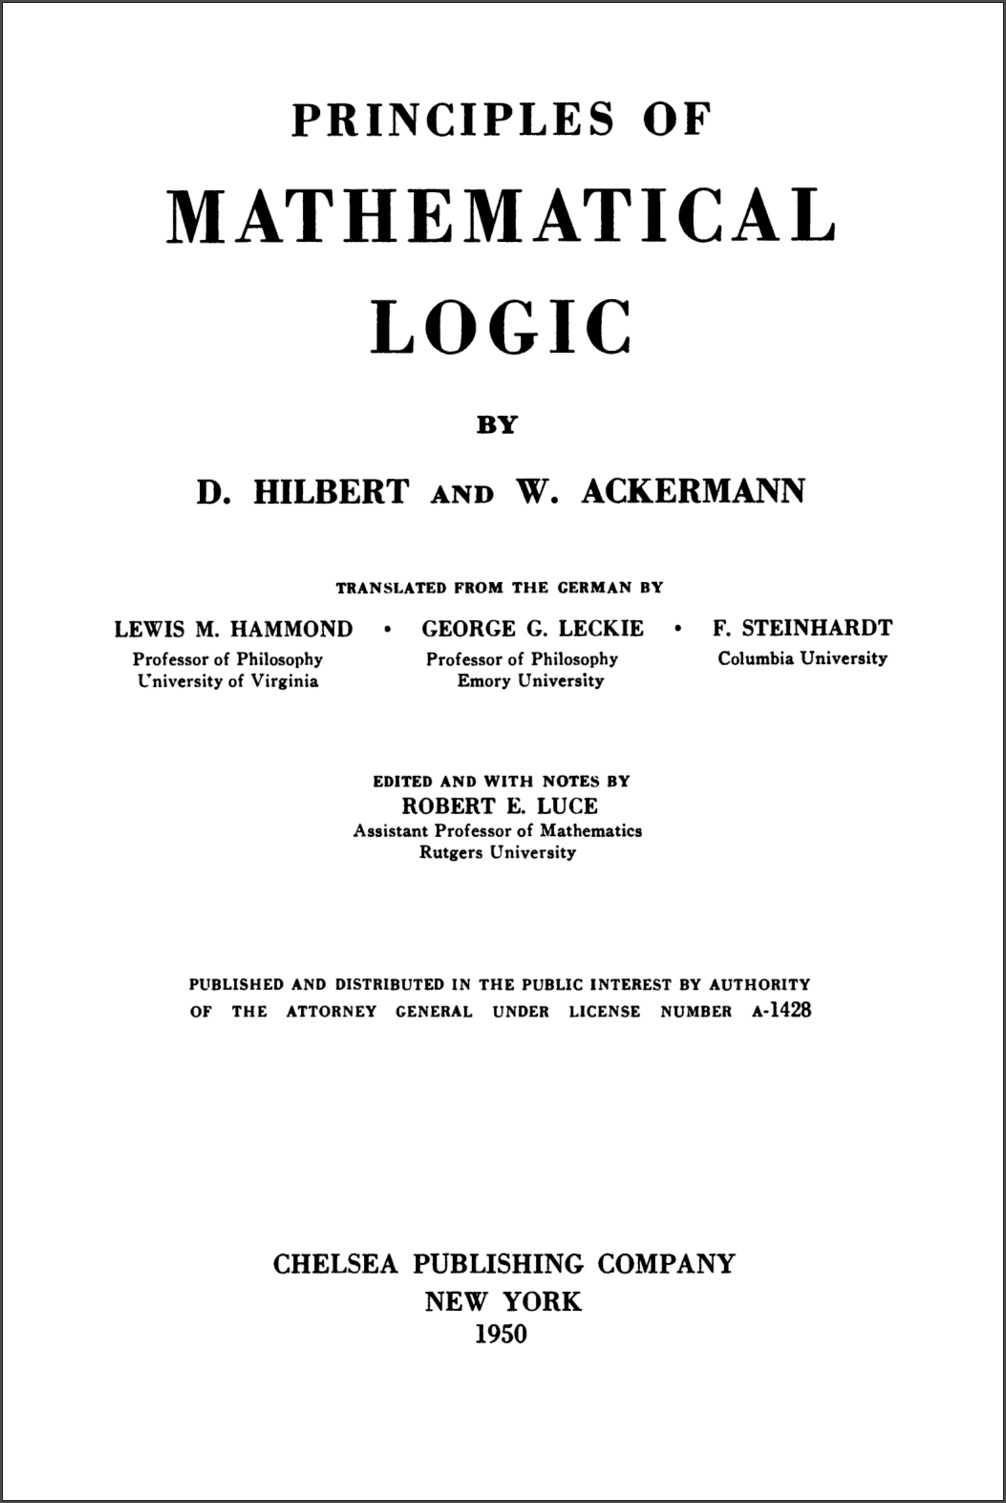
\includegraphics[width=0.443\linewidth]{img/hilbert3.png}
  \hfill
  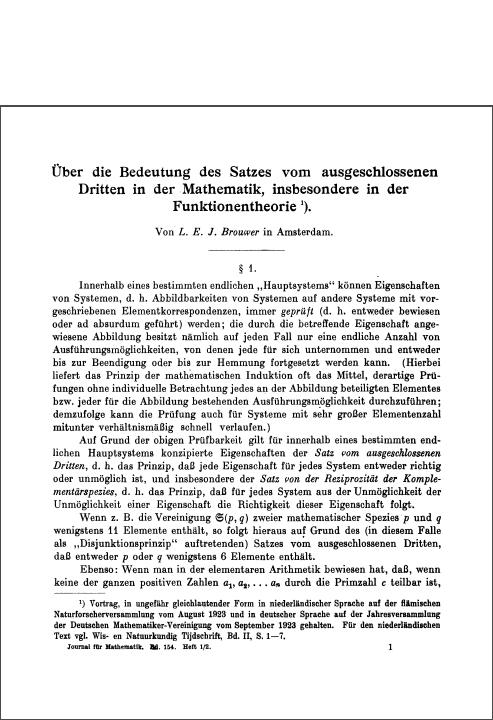
\includegraphics[width=0.53\linewidth]{img/brouwer3.png}
\begin{figure}
  \onslide<2-> 
  \begin{tikzpicture}[overlay]
  
  \node at (-3.6,5.2) {\fcolorbox{yellow}{yellow}{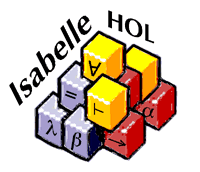
\includegraphics[scale=0.7]{img/isabelle_hol.png}}};
  
  \node at (3.3,5.2) 
  {\fcolorbox{yellow}{yellow}{ 
\includegraphics[scale=8.5]{img/coq_logo.png}}};
  
  \end{tikzpicture}
\end{figure}
\end{frame}

\begin{frame}{Outline}
  \tableofcontents
  % You might wish to add the option [pausesections]
\end{frame}

% Section and subsections will appear in the presentation overview
% and table of contents.
\section{Foundations of Formal Approach}

\subsection{A formal system}

\begin{frame}{Elements of a Formal System}%{Elements}

%\setlength{\tabcolsep}{0pt}
%\setlength\extrarowheight{0pt}
%\begin{tabular}{p{0.3\textwidth}p{0.7\textwidth}}

\begin{itemize}%[label={-}] %\setlength\itemsep{0pt}
  \item A formula (judgement, statement) $\phi \in \Phi$: 
  \begin{align*} \phi := \ & p \ | \ q \ | \ ... \ \\ 
  & | \ \phi_1 \land \phi_2 \ | \ \phi_1 \lor \phi_2 \ | \ \neg \phi_1 \ | \ \phi_1 \rightarrow \phi_2 \\
  & | \ true \ | \ false \\
  & | \ ... 
  \end{align*}
  
\def\arraystretch{0.5}
\begin{tabular}{p{0.41\textwidth} p{0\textwidth} p{0.7\textwidth}}  
  \item Propositional variables: & \item[$-$] & \item[] $p, q, ... \in V$
  \\
  \item An axiom & \item[$-$] & \item[] $\phi_{A} \in A$ %a judgement evidently claimed to be true
  \\
  \item An inference rule $\tau$ & \item[$-$] & \item[] a transition function $\tau: \Phi \rightarrow \Phi$
  \\
  \item A formula $\phi$ provable from $\Phi$ & \item[$-$] & \item[] $\Phi \vdash \phi$
  \\
  \item A tautology $\top$ & \item[$-$] & \item[] $\vdash \phi$
  \\
  \item A contradiction $\bot$ & \item[$-$] & \item[] $\vdash \neg \phi$
\end{tabular}
\end{itemize}
\end{frame}


\begin{frame}{Definition of the formal system}

A \textit{formal system} is a quadruple $\Gamma = \ <A, V, \Omega, R>$, where
\begin{itemize}
  \item $A$ -- set of axioms
  \item $V$ -- set of propositional variables
  \item $\Omega$ -- set of logical operators
  \item $R$ -- set of inference rules
\end{itemize} 

\vspace{15pt}

A \textit{formal proof} of the formula $\phi$ is a finite sequence of judgements 
\begin{align*}
\psi_1 \xrightarrow{\tau_1} \psi_2 \xrightarrow{\tau_2} ... \xrightarrow{\tau_n} \psi_n 
\end{align*}
where each $\psi_i$ is either an axiom $\phi_{A_i}$, or a formula inferred from the set of previously derived formulas according the rules of inference.


\end{frame}


%\subsection{Properties of a Formal System}
\begin{frame}{Properties of a formal system}

A formal system $\Gamma$ is called:
\begin{itemize}
\item  \textit{consistent}, \ \ \ \ if $\nexists \phi \in \Gamma: \ \Gamma \vdash \phi \land  \Gamma \vdash \neg \phi  \ \Leftrightarrow \ \Gamma \nvdash \bot$; 
\\ \vspace{3pt}
\item \textit{complete}, \ \ \ \ \ if $\forall \phi \in U: \ A \vdash \phi \lor A \vdash \neg \phi$;
\\ \vspace{3pt}
\item \textit{independent}, \ if $\not \exists a \in A: \ A \vdash a$.
\end{itemize}

\end{frame}


\subsection{Classical and Intuitionistic logics}
%\begin{theorem}
%\begin{equation}
%\exists x,y \in \mathbb{I}: \ x^{y} \in \mathbb{Q}
%\end{equation}
%\end{theorem}

\begin{frame}{Classical Logic}
{example: The Hilbert System}

%\vspace{10pt}
\textcolor{dkblue}{Set of axioms:}
%\noindent \newline
%\begin{minipage}{0.8\linewidth}
\begin{gather}
A \rightarrow (B \rightarrow A)
\tag{A1} \\
(A \rightarrow (B \rightarrow C)) \rightarrow ((A \rightarrow B) \rightarrow (A \rightarrow C))
\tag{A2} \\
A \lor \neg A
\tag{EM} 
\end{gather}
%\end{minipage}

\textcolor{dkblue}{Single inference rule (\textit{Modus Ponens})}
%q\noindent \newline
%\begin{minipage}{0.8\linewidth}
\begin{gather} 
[\![ A, A \rightarrow B ]\!] \longrightarrow B
\tag{MP}
\end{gather}
%\end{minipage}

\textcolor{dkblue}{Some provable tautologies:}
\begin{tabular}{p{.32\linewidth}p{.17\linewidth} p{.32\linewidth}p{.18\linewidth}}
$\neg \neg (A \lor \neg A)$ & (nnEM) & $\neg (A \land B) \rightarrow \neg A \lor \neg B $ & (DMdi) \\
$A \rightarrow \neg \neg A$ & (DNi)  & $\neg (A \lor B) \rightarrow \neg A \land \neg B $ & (DMci) \\
$\neg \neg A \rightarrow A$ & (DNe)  & $\neg A \land \neg B \rightarrow  \neg (A \lor B) $ & (DMce) \\
%$(A \rightarrow B) \rightarrow (\neg B \rightarrow \neg A)$ & (CP) &  
$((A \rightarrow B) \rightarrow A) \rightarrow B$ & (PL) & $\neg A \lor \neg B \rightarrow  \neg (A \land B) $ & (DMde)
\end{tabular}

\end{frame}


\begin{frame}{Intuitionistic Logic}
{a.k.a. Constructive Logic}

%\vspace{10pt}
\textcolor{dkblue}{Set of axioms:}
\begin{gather}
A \rightarrow (B \rightarrow A)
\tag{A1} \\
(A \rightarrow (B \rightarrow C)) \rightarrow ((A \rightarrow B) \rightarrow (A \rightarrow C))
\tag{A2} \\
\hcancel[red]{ A \lor \neg A }
\tag{EM} 
\end{gather}

\textcolor{dkblue}{Single inference rule (\textit{Modus Ponens})}
\begin{gather} 
[\![ A, A \rightarrow B ]\!] \longrightarrow B
\tag{MP}
\end{gather}
%\vspace{5pt}
\textcolor{dkblue}{Some provable tautologies:}

\begin{tabular}{p{.32\linewidth}p{.2\linewidth} p{.3\linewidth}p{.25\linewidth}}
  $\neg \neg (A \lor \neg A)$ & (nnEM) & $\hcancel[red]{ \neg (A \land B) \rightarrow \neg A \lor \neg B }$ & (DMdi) \\
  $A \rightarrow \neg \neg A$ & (DNi)  & $\neg (A \lor B) \rightarrow \neg A \land \neg B $ & (DMci) \\
  $\hcancel[red]{ \neg \neg A \rightarrow A }$ & (DNe)  & $\neg A \land \neg B \rightarrow  \neg (A \lor B) $ & (DMce) \\
  %$(A \rightarrow B) \rightarrow (\neg B \rightarrow \neg A)$ & (CP) &  
  $\hcancel[red]{ ((A \rightarrow B) \rightarrow A) \rightarrow B }$ & (PL) & $\neg A \lor \neg B \rightarrow  \neg (A \land B) $ & (DMde)
\end{tabular}

\end{frame}

\begin{frame}<presentation:0>{Curry-Howard Correspondence}

The direct relationship between computer programs and mathematical proofs.

[To be done]
\end{frame}


\section{Two Theorem Provers}

\subsection{Isabelle \& Coq}

\begin{frame}[fragile]{Isabelle \& Coq} {First acquaintance}
%\vspace{3pt}
\begin{tabular}{@{} p{.45\linewidth} @{\hspace{8pt}}|@{\hspace{8pt}} p{0.56\linewidth} @{}} %{p{.47\linewidth} @{\hspace{8pt}}|@{\hspace{8pt}} p{.49\linewidth}}
\begin{center} 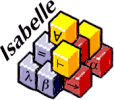
\includegraphics[scale=0.5]{img/isabelle_logo.png} \end{center} & \begin{center} 
\includegraphics[scale=4]{img/coq_logo.png} \end{center} \\

% --
\textcolor{ltdkblue}{$\bullet$} based on \textbf{classical} higher-order logic &
\textcolor{ltdkblue}{$\bullet$} based on \textbf{intuitionistic} logic \newline \textcolor{dkgray}{ (Calculus of Inductive Constructions) } \\

& \\[0.8em] % Empty table row with custom line break spacing.

\textcolor{ltdkblue}{$\bullet$} created in 1986 at University of Cambridge and Technische Universit\"{a}t M\"{u}nchen &

\textcolor{ltdkblue}{$\bullet$} created in 1984 at INRIA \newline (Paris, France) \\

& \\[0.8em]

\textcolor{ltdkblue}{$\bullet$} \textcolor{dkgray}{ uses functional language \texttt{HOL} } &
\textcolor{ltdkblue}{$\bullet$} \textcolor{dkgray}{ uses functional language \texttt{Gallina} } \\

& \\[0.8em]

\textcolor{ltdkblue}{$\bullet$} \textcolor{dkgray}{ has large collection of formalised \newline theories } & 
\textcolor{ltdkblue}{$\bullet$} \textcolor{dkgray}{ has large collection of formalised \newline theories }

\end{tabular} 

\end{frame}


\begin{frame}[fragile]{Isabelle \& Coq} {Definition of the basic datatypes}
\vspace{-12.5pt}
\begin{tabular}{@{} p{.45\linewidth} @{\hspace{8pt}}|@{\hspace{8Pt}} p{0.56\linewidth} @{}}
  \begin{center} 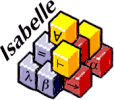
\includegraphics[scale=0.5]{img/isabelle_logo.png} \end{center} & \begin{center} 
\includegraphics[scale=4]{img/coq_logo.png} \end{center} \\
\onslide<2->
\begin{lstlisting}[language=isabelle]
datatype bool = 
  True | False

datatype nat = 
  zero ("0") | Suc nat
\end{lstlisting}
&
\onslide<3->
\begin{lstlisting}[language=coq]
Inductive False : Prop := .

Inductive True : Prop := I : True.

Inductive nat : Type :=
  | O : nat
  | S : nat -> nat.
\end{lstlisting}
\end{tabular}
%\end{raggedleft}

\end{frame}


\begin{frame}[fragile]{Isabelle \& Coq} {Definition of a recursive function}
%\vspace{3pt}
\vspace{-4.5pt}
\begin{tabular}{@{} p{.45\linewidth} @{\hspace{8pt}}|@{\hspace{8pt}} p{0.56\linewidth} @{}}
  \begin{center} 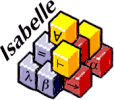
\includegraphics[scale=0.5]{img/isabelle_logo.png} \end{center} & \begin{center} 
\includegraphics[scale=4]{img/coq_logo.png} \end{center} \\

\onslide<2->
\begin{lstlisting}[language=isabelle]
fun add :: 
  "nat => nat => nat"
where
  "add 0 n = n"
  
  | "add (Suc m) n =
       Suc(add m n)"
\end{lstlisting}
&
\onslide<3->
\begin{lstlisting}[language=coq]
Fixpoint add (n m: nat) : nat :=
  match n with
    | O => m
    | S n' => S (n' + m)
end

where "n + m" :=
  (add n m) : nat_scope.
\end{lstlisting}
\end{tabular}
\end{frame}


\begin{frame}[fragile]{Isabelle: Native graphical user interface}
\begin{center}
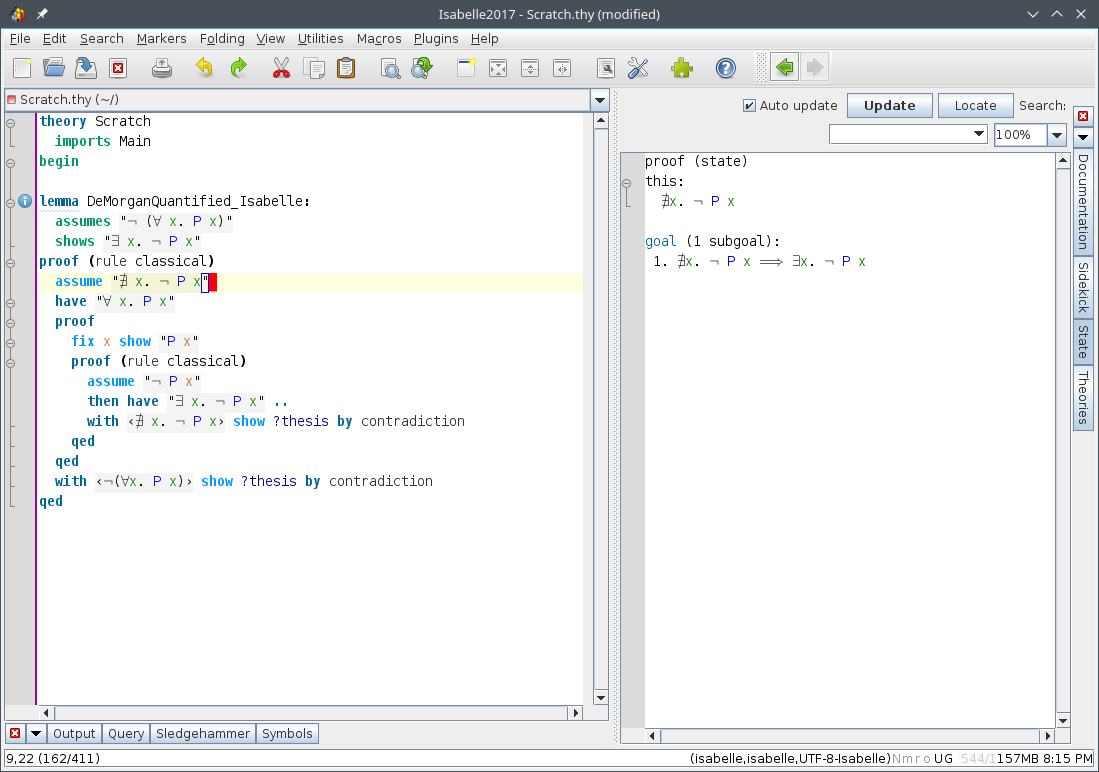
\includegraphics[scale=0.4]{img/isabelle_morgan.png}
\end{center}
\end{frame}

\begin{frame}[fragile]{Coq: Native graphical user interface}
\begin{center}
  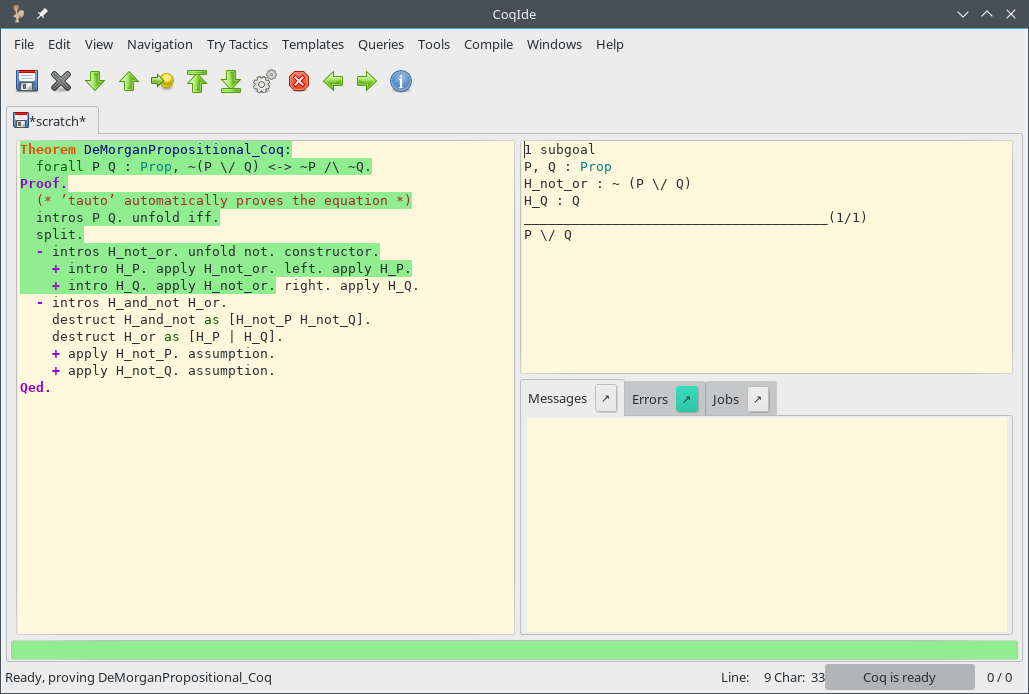
\includegraphics[scale=0.42]{img/coq_morgan.png}
\end{center}
\end{frame}

\section{Comparison of the theorem provers}

\subsection{Comparison}

\begin{frame}{Comparison}
\textcolor{dkblue}{Major similarities:}
\begin{itemize}
  \item both work in a similar way of \textit{verifying} the proof or \textit{assisting} in creation of the new one
  \item \textit{premises} $\xrightarrow{tactics}$ \textit{goals} (forward proof)
  \item \textit{goals} $\xrightarrow{tactics}$ \textit{premises} (backward proof)
  \item both have large amount of libraries with formalised theories
  \item both dispose the set of highly automated tactics
  \item both are being actively developed these days
\end{itemize}

\vspace{10pt}
\textcolor{dkblue}{Major differences:}
\begin{itemize}
  \item based on different logics $\Rightarrow$
  \begin{itemize}
    \item[$\star$] unprovable statements and invalid proofs in Coq
    \item[$\star$] sometimes more complex proof in Coq
    \item[$\star$] \textit{constructive} proof in Coq
    
  \end{itemize}
\end{itemize}

\end{frame}


\subsection{Proof examples}

\begin{frame}
%<presentation:0>
{Isabelle: proof example in propositional logic}
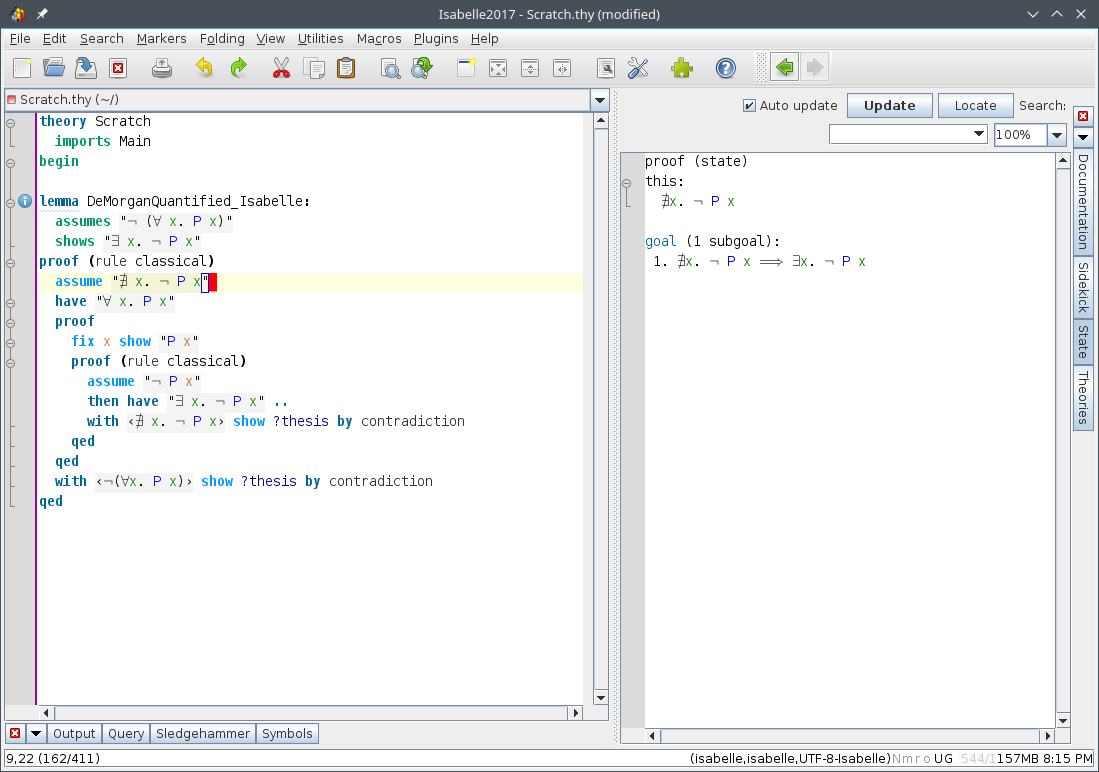
\includegraphics[scale=0.39]{img/isabelle_morgan.png}
\end{frame}

\begin{frame}{Isabelle: proof example over \texttt{nat}}
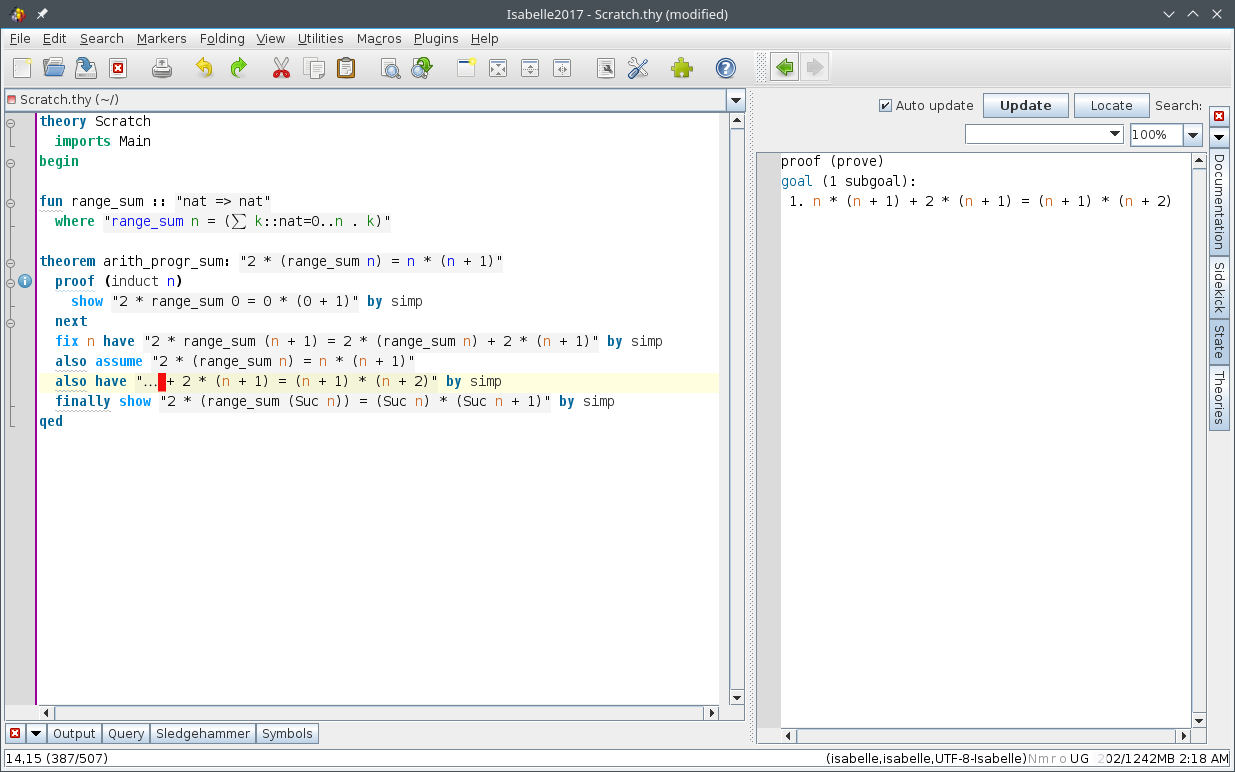
\includegraphics[scale=0.39]{img/isabelle_arith.png}
\end{frame}



\begin{frame}
%<presentation:0>
{Coq: proof example in propositional logic}
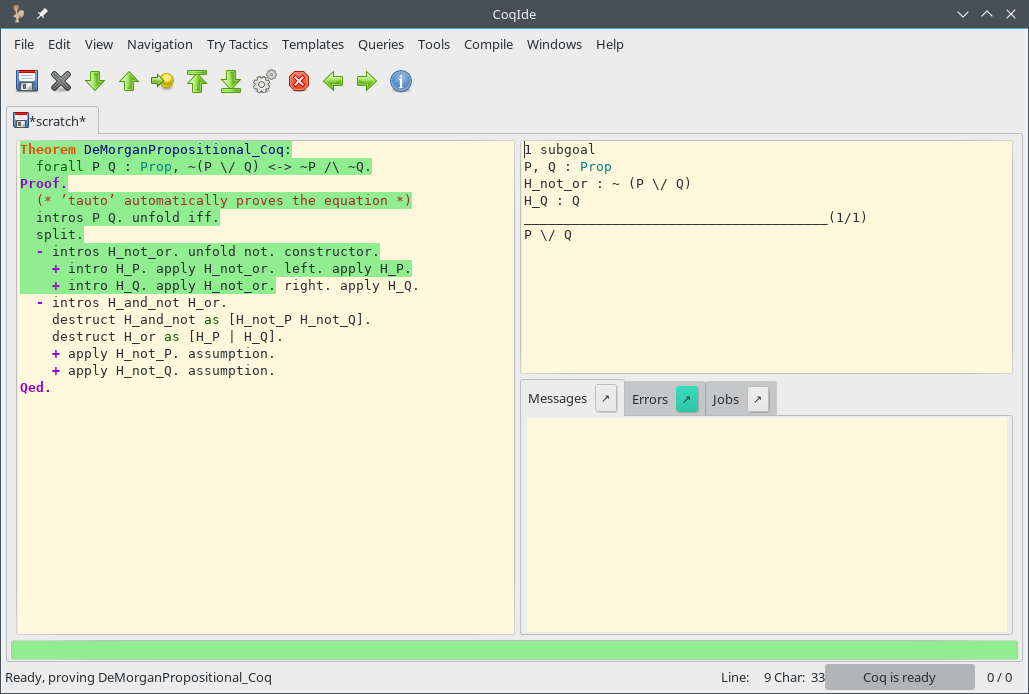
\includegraphics[scale=0.42]{img/coq_morgan.png}
\end{frame}

\begin{frame}{Coq: proof example over \texttt{nat}}
%\animategraphics[loop,controls,width=\linewidth]{3}{img/gif-coq/gif/something}{0}{21}
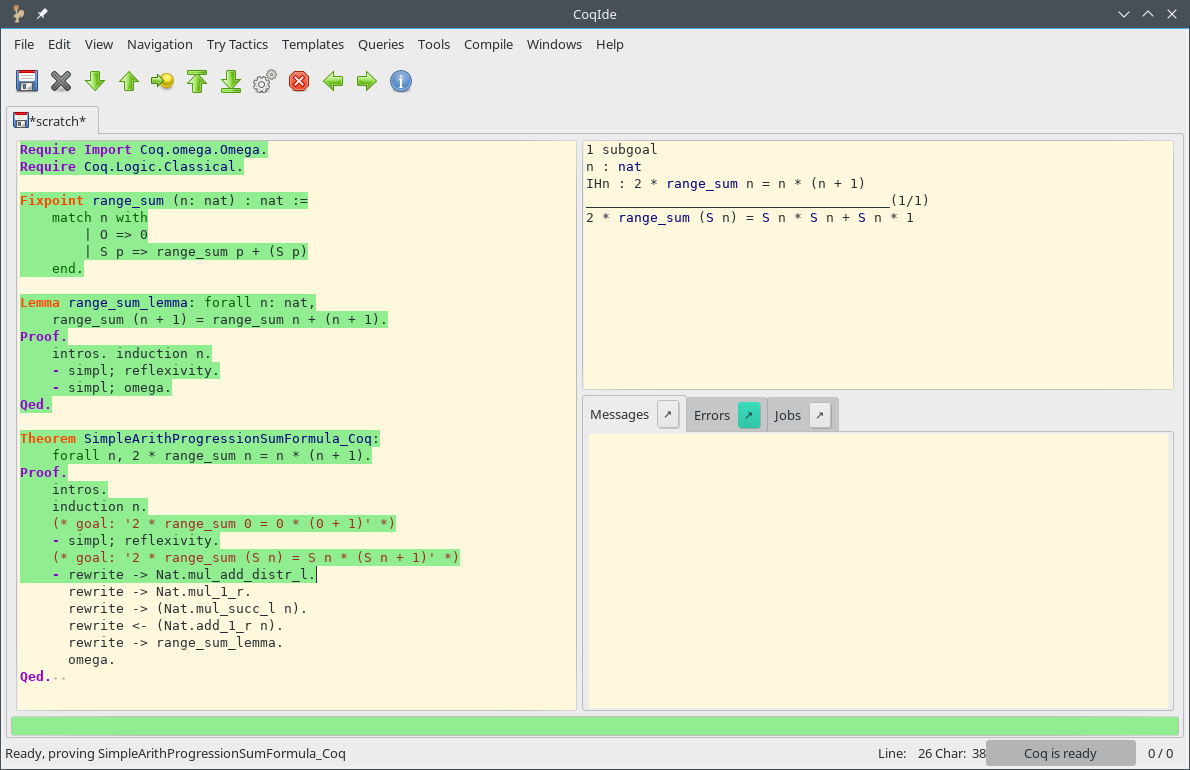
\includegraphics[scale=0.39]{img/gif-coq/coq-arith-6.png}
\end{frame}


\begin{frame}{Coq: proof example over \texttt{nat} + verified code extraction}
%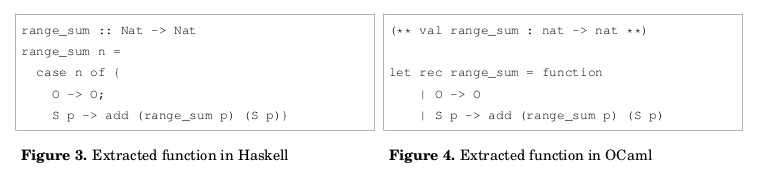
\includegraphics[scale=0.39]{img/coq_extract.png}
%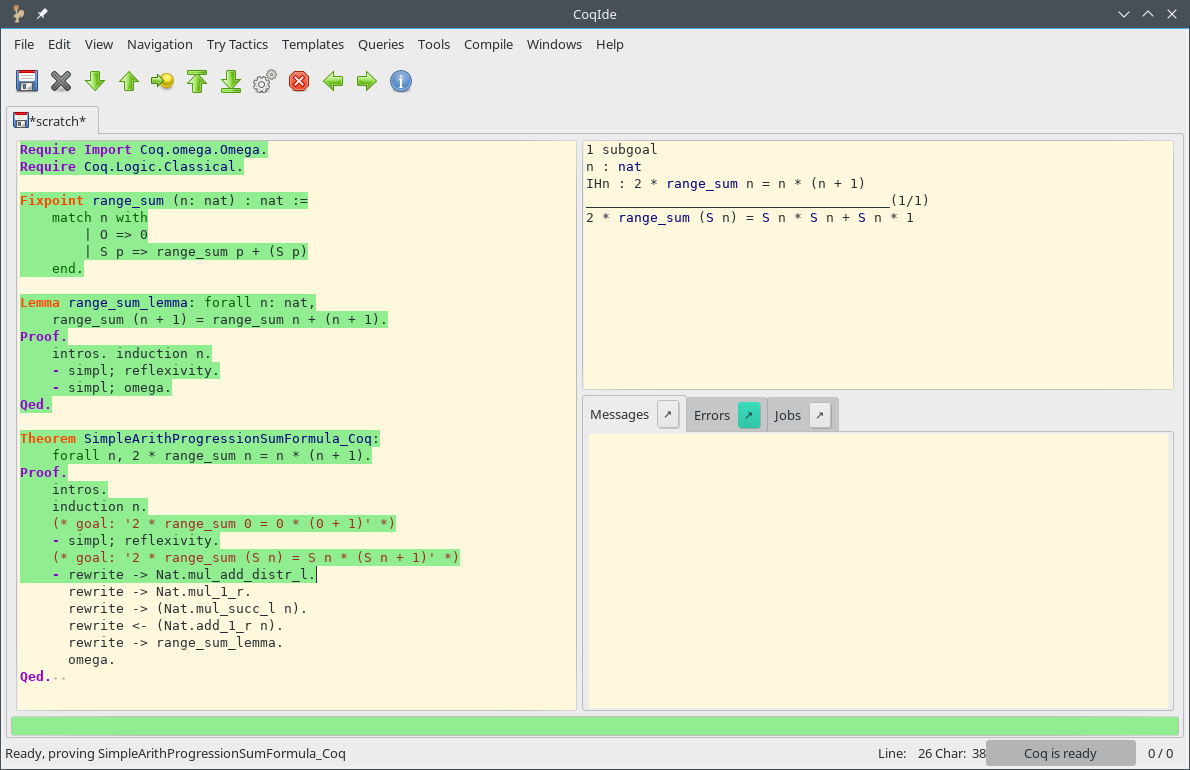
\includegraphics[scale=0.39]{img/gif-coq/coq-arith-6.png}

\begin{figure}
  \begin{tikzpicture}[overlay]
  \node at (-0.36,-0.44) {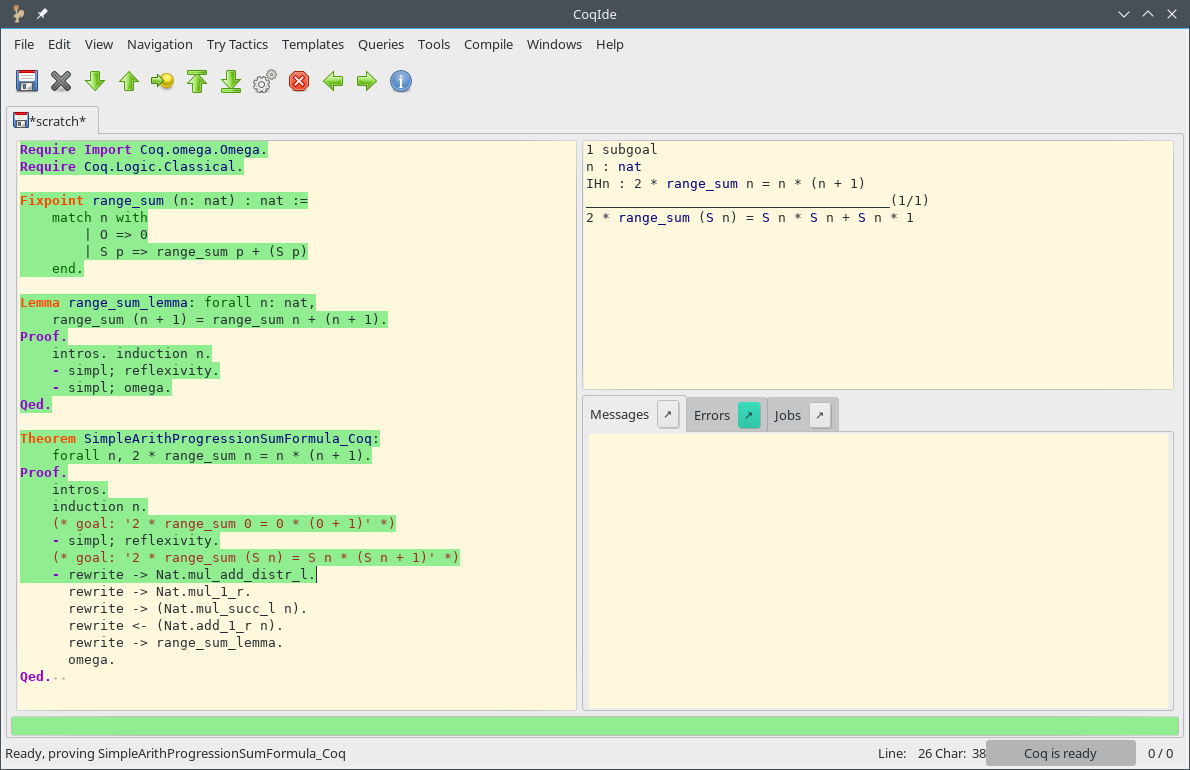
\includegraphics[scale=0.39]{img/coq_arith.png}};
  \node at (0.25,0.1) {\fcolorbox{yellow}{yellow}{ 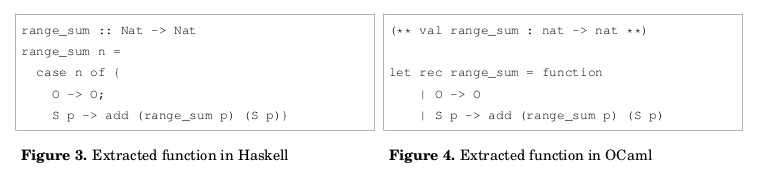
\includegraphics[scale=0.5]{img/coq_extract.png}} };
  \end{tikzpicture}
\end{figure}

\end{frame}


%\begin{frame}{Blocks}
%\begin{block}{Block Title}
%You can also highlight sections of your presentation in a block, with it's own title
%\end{block}
%\begin{theorem}
%There are separate environments for theorems, examples, definitions and proofs.
%\end{theorem}
%\begin{example}
%Here is an example of an example block.
%\end{example}
%\end{frame}

% Placing a * after \section means it will not show in the
% outline or table of contents.
\section*{Summary}

\begin{frame}{Summary}
  \begin{itemize}
  \item
    Two widespread theorem provers were considered: \textcolor{dkblue}{Isabelle} and \textcolor{dkblue}{Coq}
  \item
    The \textcolor{dkblue}{key difference} between them lie in differences between logical theories
    they based on
  \item
    Nonetheless, they both may be used to solve applied problems, such as software testing and verification
  \end{itemize}
  
%\begin{itemize}
%\item
%  Outlook
%  \begin{itemize}
%  \item
%    Something you haven't solved.
%  \item
%    Something else you haven't solved.
%  \end{itemize}
%\end{itemize}

\end{frame}



% All of the following is optional and typically not needed. 
\appendix
\section<presentation>*{\appendixname}
\subsection<presentation>*{For Further Reading}

%\begin{frame}[allowframebreaks]
%  \frametitle<presentation>{For Further Reading}
%    
%  \begin{thebibliography}{10}
%    
%  \beamertemplatebookbibitems
%  % Start with overview books.
%
%  \bibitem{Author1990}
%    A.~Author.
%    \newblock {\em Handbook of Everything}.
%    \newblock Some Press, 1990.
% 
%    
%  \beamertemplatearticlebibitems
%  % Followed by interesting articles. Keep the list short. 
%
%  \bibitem{Someone2000}
%    S.~Someone.
%    \newblock On this and that.
%    \newblock {\em Journal of This and That}, 2(1):50--100,
%    2000.
%  \end{thebibliography}
%\end{frame}


\end{document}


